\documentclass[conference]{IEEEtran}

\usepackage{amsmath,amsthm,amssymb}
\usepackage{graphicx}
\usepackage{subfigure}

\usepackage{url}
\usepackage{cite}

% correct bad hyphenation here
\hyphenation{op-tical net-works semi-conduc-tor}

\begin{document}

\title{Traf: A Camera Based System for Traffic Flow Analysis}
\maketitle
\author{fsb}

\begin{abstract}

In this paper, we present a camera based system(Traf) to count automotive vehicles for traffic flow analysis use. The system employs the method of background subtraction by comparing differences between foreground and background. The background model is initialed by averaging first 50 frames, and adapted to environment change by introducing an adapting parameter $\lambda$. Compared to state-of-art method, it is more robust, adaptive and economical.

\end{abstract}


%--------------------------------------------------------------------------------
% what and why ?
\section{Introduction}

%================================================================================

% how?
\section{System Design}
	\subsection{Overview}
	The system consists of 3 main modules, video collector, vehicle counter and flow analyzer as Fig \ref{fig:sysDiagram}. Video collector is designed to collect the original video sources and transform them into a unified format for further use. Flow analyzer is designed to calculate the result and provide suggestion for traffic use. The vehicle counter is the core module of the system, which is further divided into 4 steps as, detector, tracker, follower and generator. 
	
	\begin{figure}[!h]
	\centering
	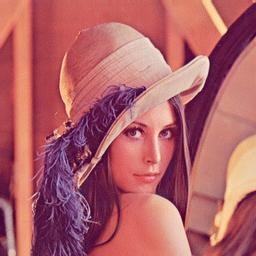
\includegraphics[width=0.8\linewidth]{figures/lena.jpg} 
	\caption{System diagram}
	\label{fig:sysDiagram}
	\end{figure}
	
	%============================================================================
	\subsection{Background Subtraction}
	As the monitoring camera is deployed with a fixed position, videos collected from this kind of devices would have a stable background. And the automobile vehicles forms the foreground motions. Hence, content of each frame image contains two parts, foreground and background. To detect the vehicles, we utilize background subtraction method, which can be described as:
	\begin{equation}
	M_{mask} = F_{foreground}  - B_{background}
	\end{equation}
	Where $F_{foreground}$ and $B_{background}$ are derived from foreground and background images correspondingly, and $M_{mask}$ is the mask of detected foreground mask.
	
	Frame images from video usually have more than one channel, and they may vary from different types and sizes. This makes it hard or impossible for directing subtraction calculation. Hence, we introduce a collector module to unify the original frame images, as Fig. \ref{fig:unifyDiagram}
	\begin{figure}[!h]
	\centering
	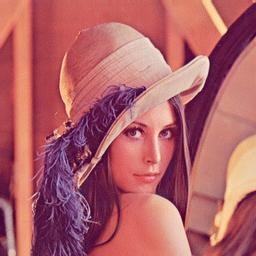
\includegraphics[width=0.8\linewidth]{figures/lena.jpg} 
	\caption{Frame image unifying}
	\label{fig:unifyDiagram}
	\end{figure}
		
	
	\subsection{Background Model}
	\subsection{Motion Detection and Tracking}
	\subsection{Traffic Flow Analysis}
	
	
	
% compare and check	
\section{Implementation and Evaluation}
	\subsection{Setup}
	\subsection{Methodology}
	\subsection{Result}



\section{Conclusion}


\end{document}